\documentclass[11pt,a4paper]{article}

\usepackage[margin=2.3cm]{geometry}
\usepackage[T1]{fontenc}
\usepackage{lmodern}
\usepackage{graphicx}
\usepackage{booktabs}
\usepackage{amsmath,amssymb}
\usepackage{xcolor}
\usepackage{float}
\usepackage{caption}
\usepackage{subcaption}
\usepackage{tikz}
\usetikzlibrary{positioning,arrows.meta,shapes.geometric}
\usepackage{enumitem}
\usepackage{hyperref}
\hypersetup{colorlinks=true,linkcolor=blue!50!black,urlcolor=blue!50!black,citecolor=blue!50!black}
\graphicspath{{figures/}}
\setlength{\parskip}{4pt}
\setlength{\parindent}{0pt}
\captionsetup{font=small,labelfont=bf}

\newcommand{\code}[1]{\texttt{#1}}

\title{\textbf{Lumina CV: Noise- and Temporal-Aware\\Zero-Reference Low-Light Image Enhancement}\\[4pt]
\large Project Report}
\author{
\begin{tabular}{ll}
Jatin Purbia & B23CH11022\\
Sharana Gouda Lakshetty & B23CH1042\\
Rahul Ahuja & B23CH1037
\end{tabular}}
\date{November 2026}

\begin{document}
\maketitle

\begin{abstract}
We built Lumina CV, an end-to-end system for brightening photographs taken in poor light. It has three parts: a PyTorch model (``NTA-ZeroDCE''), a FastAPI inference server and a Next.js web application that shows a before/after comparison with an in-browser quality analysis. The model extends Zero-Reference Deep Curve Estimation (Zero-DCE) with a noise-estimation branch, a residual denoiser, and extra losses for edges, chromaticity and adaptive exposure. It also has an optional video-consistency path that uses optical flow. It is trained without any paired ground truth.

This report describes the method and the software, and it analyses the training settings we tried while looking for the best model. We evaluated all eight saved training checkpoints (epochs 5 to 40) and four inference settings on the 15 held-out LOL image pairs. We also compared the model against plain gamma correction and histogram equalisation. The main finding is a trade-off. Held-out PSNR rises from 10.7~dB (epoch 10) to 16.6~dB (epoch 40), but the model drifts towards brightening everything too much, so ordinary photographs wash out. We therefore ship the 10-epoch model. Gamma correction with $\gamma=0.3$ reaches 16.7~dB PSNR, higher than any checkpoint, so the model's advantage is in colour fidelity and noise behaviour rather than pixel-wise PSNR. The 13-row ablation matrix was implemented but not run, so we make no ablation claims.
\end{abstract}

\tableofcontents
\newpage

%--------------------------------------------------------------------
\section{Introduction}
Photographs taken in low light are dark, noisy and low in contrast. Brightening them is simple to state but hard to do well: a global brightness boost lifts the noise as much as the signal, and it can blow out regions that were already well exposed. Learning-based enhancers address this but usually need paired dark/bright images, which are expensive to collect and tie the model to one camera.

\textbf{Zero-DCE}~\cite{zerodce} avoids paired data. A small network predicts, for every pixel, the parameters of a brightness curve. The curve is applied several times to the input. Training uses only hand-designed losses (exposure, colour constancy, spatial consistency, smoothness) computed on the output itself. The network is tiny (about 1~MB here) and fast.

Our goals were:
\begin{enumerate}[nosep]
  \item Re-implement the Zero-DCE idea cleanly, with a strict configuration system and a large automated test-suite.
  \item Add \emph{noise awareness}, so that dark regions are not brightened into visible noise, and a light denoiser.
  \item Add edge, chromaticity and adaptive-exposure losses, and an optional temporal-consistency mechanism for video.
  \item Wrap the model in an HTTP API and a web application anyone can use, with an in-browser analysis of what the enhancement did.
  \item Find a training recipe that gives natural results, and document honestly what worked and what did not.
\end{enumerate}

\textbf{Contributions.} (i) The NTA-ZeroDCE model and training code; (ii) a deployable API and web app; (iii) an evaluation of the training schedule, baselines and inference settings, including the finding that longer training over-brightens ordinary photos while improving the standard benchmark score.

%--------------------------------------------------------------------
\section{Method}
\subsection{Notation and curve model}
Images are RGB tensors with values in $[0,1]$. The network $\mathcal{F}$ predicts eight curve-parameter maps $A_1,\dots,A_8$ (each with three channels, so 24 output channels, passed through $\tanh$ to lie in $[-1,1]$). The input $x_0=x$ is brightened by iterating the quadratic curve
\begin{equation}
  x_{i+1} = x_i + A_i \odot x_i \odot (1-x_i), \qquad i=0,\dots,7 .
\end{equation}
The curve fixes the end points $0$ and $1$ for any $A$, and $A=0$ is the identity (Fig.~\ref{fig:curves}). Positive $A$ brightens, negative $A$ darkens, and because $A$ varies per pixel the enhancement is spatially adaptive.

\begin{figure}[H]
  \centering
  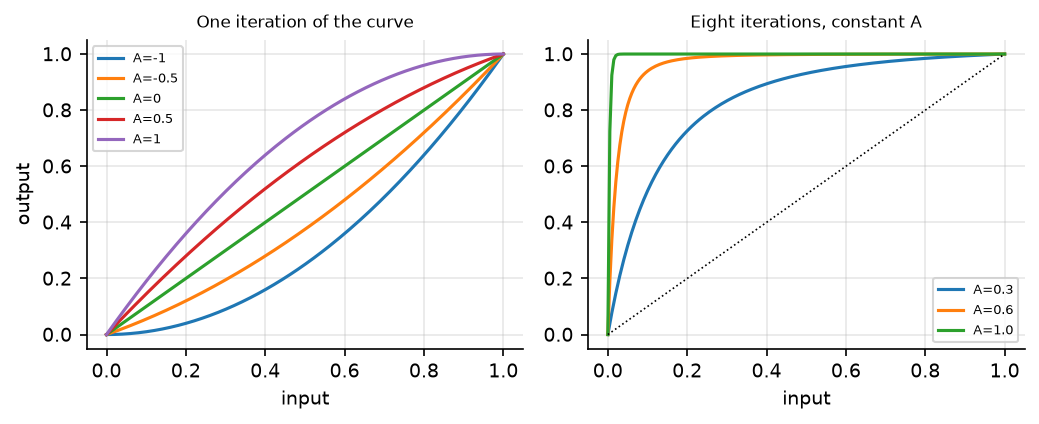
\includegraphics[width=.7\linewidth]{curves.png}
  \caption{The light-enhancement curve. Left: one iteration for several values of $A$. Right: eight iterations with a constant $A$ give a strong, smooth tone-mapping that never leaves $[0,1]$.}
  \label{fig:curves}
\end{figure}

\subsection{Network architecture}
Fig.~\ref{fig:arch} shows the pipeline. All components are small convolutional networks.

\begin{figure}[H]
\centering
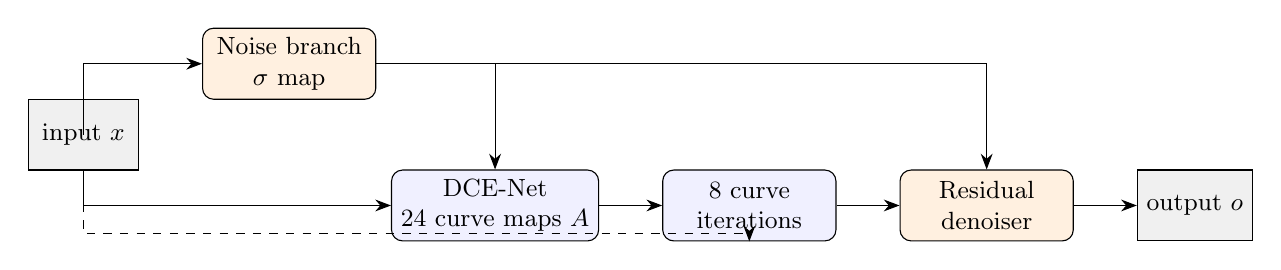
\begin{tikzpicture}[node distance=7mm and 8mm, every node/.style={font=\small},
  box/.style={draw,rounded corners,minimum height=9mm,minimum width=22mm,align=center,fill=blue!6},
  opt/.style={draw,rounded corners,minimum height=9mm,minimum width=22mm,align=center,fill=orange!12},
  io/.style={draw,minimum height=9mm,minimum width=14mm,align=center,fill=gray!12},
  arr/.style={-{Stealth[length=2mm]}}]
 \node[io] (x) {input $x$};
 \node[opt,right=of x,yshift=9mm] (nb) {Noise branch\\$\sigma$ map};
 \node[box,right=of x,yshift=-9mm,xshift=24mm] (dce) {DCE-Net\\24 curve maps $A$};
 \node[box,right=of dce] (cur) {8 curve\\iterations};
 \node[opt,right=of cur] (den) {Residual\\denoiser};
 \node[io,right=of den] (o) {output $o$};
 \draw[arr] (x) -- ++(0,0) |- (nb);
 \draw[arr] (x) |- (dce);
 \draw[arr] (nb) -| (dce);
 \draw[arr] (dce) -- (cur);
 \draw[arr] (cur) -- (den);
 \draw[arr] (den) -- (o);
 \draw[arr] (nb.east) -- ++(48mm,0) -| (den.north);
 \draw[arr,dashed] (x.south) -- ++(0,-8mm) -| (cur.south);
\end{tikzpicture}
\caption{NTA-ZeroDCE. Orange blocks (noise branch, denoiser) are optional extensions; with them disabled the model is the Zero-DCE baseline. The dashed arrow shows that the curves are applied to the original input.}
\label{fig:arch}
\end{figure}

\begin{itemize}[nosep]
  \item \textbf{DCE-Net.} Seven $3\times3$ convolutions with 32 channels, ReLU, symmetric skip connections ($h_3\!+\!h_4$, $h_2\!+\!h_5$, $h_1\!+\!h_6$) and a $\tanh$ head. No normalisation or down-sampling.
  \item \textbf{Noise branch.} Three convolutions (RGB $\to$ 16 $\to$ 16 $\to$ 1) with a sigmoid scaled to $[0,0.2]$; it predicts a per-pixel noise level $\sigma$, which is concatenated to the DCE-Net input.
  \item \textbf{Residual denoiser.} Two depthwise/pointwise 16-channel blocks. Its input is the curve output $z$ plus $\sigma\cdot G$, where $G=\mathrm{clamp}\!\big(\mathrm{avgpool}_5(Y(z))/\mathrm{avgpool}_5(Y(x)),1,8\big)$ is the local gain the curves applied (brightening amplifies noise by about that gain). The final output is $o=\mathrm{clamp}(z-0.1\tanh(\mathrm{Denoiser}(\cdot)),0,1)$.
  \item \textbf{Light variant.} An optional depthwise-separable DCE-Net and a \code{curve\_scale} option estimate the curves at reduced resolution and up-sample them, which is used in Sec.~\ref{sec:curvescale}.
\end{itemize}

\subsection{Training losses}
Training needs no reference images. The four baseline losses follow Zero-DCE:
\begin{itemize}[nosep]
  \item \textbf{spa} (weight 1): neighbouring $4\times4$-pooled contrast must be preserved between input and output.
  \item \textbf{exp} (weight 10): $\overline{(P_{16}(Y(o))-E)^2}$ pulls the mean intensity of $16\times16$ patches toward a target $E$ (the ``exposure target'').
  \item \textbf{col} (weight 5): penalises differences between the mean R, G, B channels (grey-world colour constancy).
  \item \textbf{tv} (weight 200): smoothness of the curve maps $A$.
\end{itemize}
Our extensions, each behind a feature flag in the configuration:
\begin{center}
\small
\begin{tabular}{llp{8.2cm}c}
\toprule
Flag & Loss & Idea & Weight\\
\midrule
\code{noise\_aware} & noise, invariance & Add synthetic signal-dependent noise ($\mathrm{var}=ax+b^2$) so the true $\sigma$ is known; the noisy output must match a no-gradient clean-input teacher & 20, 10\\
\code{denoise} & fidelity & Denoised output stays close to the teacher's raw output & 1\\
\code{edge} & edge & Output gradients follow gain-scaled input gradients, down-weighted where the gradient is noise & 20\\
\code{chroma} & chroma & Output chromaticity $v/\sum v$ follows the locally averaged input chromaticity (prevents colour shifts) & 20\\
\code{adaptive\_exp} & adaptive\_exp, highlight & Replaces \emph{exp} by a per-region target that rises for bright and falls for noisy regions; penalises brightening bright pixels & 10, 20\\
\code{temporal} & temporal & L1 between the output and the flow-warped previous output on reliable pixels & 10\\
\bottomrule
\end{tabular}
\end{center}
Targets, masks, $\sigma$ and the gain used inside the losses are detached. The total loss is the weighted sum of enabled terms, minimised with Adam (learning rate $10^{-4}$, weight decay $10^{-4}$, gradient clipping 0.1).

\subsection{Video consistency}
For video, an OpenCV DIS optical-flow estimator is run in both directions; a pixel is ``reliable'' if the forward/backward flows agree, the photometric difference is small and the pixel stays in bounds. At inference the curves of the current frame are blended with the warped, smoothed curves of the previous frame, $\bar A_t=(1-0.7m)A_t+0.7m\,\mathrm{warp}(\bar A_{t-1})$ with $m$ the reliability mask; a histogram-based scene-cut detector resets the state. A still image never uses flow or state. The temporal path is implemented and tested, but the shipped photo model was trained without it (see Sec.~\ref{sec:training}).

%--------------------------------------------------------------------
\section{System implementation}
\begin{figure}[H]
\centering
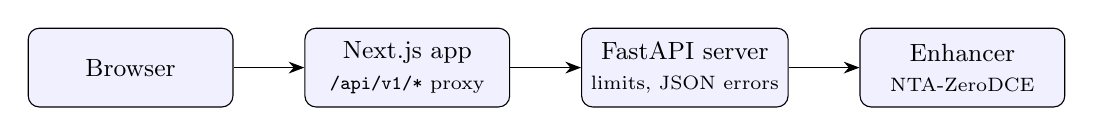
\begin{tikzpicture}[node distance=9mm, box/.style={draw,rounded corners,minimum height=10mm,minimum width=26mm,align=center,fill=blue!6,font=\small}, arr/.style={-{Stealth[length=2mm]}}]
 \node[box] (b) {Browser};
 \node[box,right=of b] (w) {Next.js app\\\scriptsize\code{/api/v1/*} proxy};
 \node[box,right=of w] (a) {FastAPI server\\\scriptsize limits, JSON errors};
 \node[box,right=of a] (m) {Enhancer\\\scriptsize NTA-ZeroDCE};
 \draw[arr] (b) -- (w); \draw[arr] (w) -- (a); \draw[arr] (a) -- (m);
\end{tikzpicture}
\caption{Deployment architecture. The web layer never runs the model; it proxies requests at run-time to the API (\code{LUMINA\_API\_URL}).}
\end{figure}
\begin{itemize}[nosep]
  \item \textbf{Python package} \code{nta\_zerodce} (\code{core/}): modules for models, losses, data, flow, inference, metrics, training, API and a shared CLI. Dependencies are one-directional (e.g.\ models never import losses or data). Experiments are Python files with a strict schema: unknown or missing keys fail, flag dependencies are checked, and each run saves its resolved \code{config.yaml}.
  \item \textbf{Scripts:} \code{train}, \code{evaluate}, \code{enhance}, \code{ablate}, \code{make\_synthetic\_data}, \code{download\_lol}.
  \item \textbf{API} (FastAPI): \code{GET /health}, \code{GET /options}, \code{POST /enhance} (PNG/JPEG upload with optional \code{curve\_scale}, returns an 8-bit PNG). Uploads are limited in bytes, pixels and side length; errors are always JSON with fixed codes; requests carry an id and \code{Cache-Control: no-store}. Checkpoint, device and limits are set through environment variables, and a Docker image is provided.
  \item \textbf{Web app} (Next.js, TypeScript): image upload with client-side validation and down-scaling, a draggable before/after slider, and an Analysis panel computed in the browser (Fig.~\ref{fig:ui}).
  \item \textbf{Quality assurance:} about 2060 Python tests (numerical identities, gradients, curve and affine conventions, checkpoint round trips, a 30-step overfit test, an end-to-end train/enhance/evaluate cycle, API contract and error codes) and a web test-suite (Vitest), plus linting, type-checking and a GitHub Actions workflow. When we re-ran the Python tests for this report: 2059 passed, 2 skipped (they need a CUDA GPU).
\end{itemize}

\begin{figure}[H]
\centering
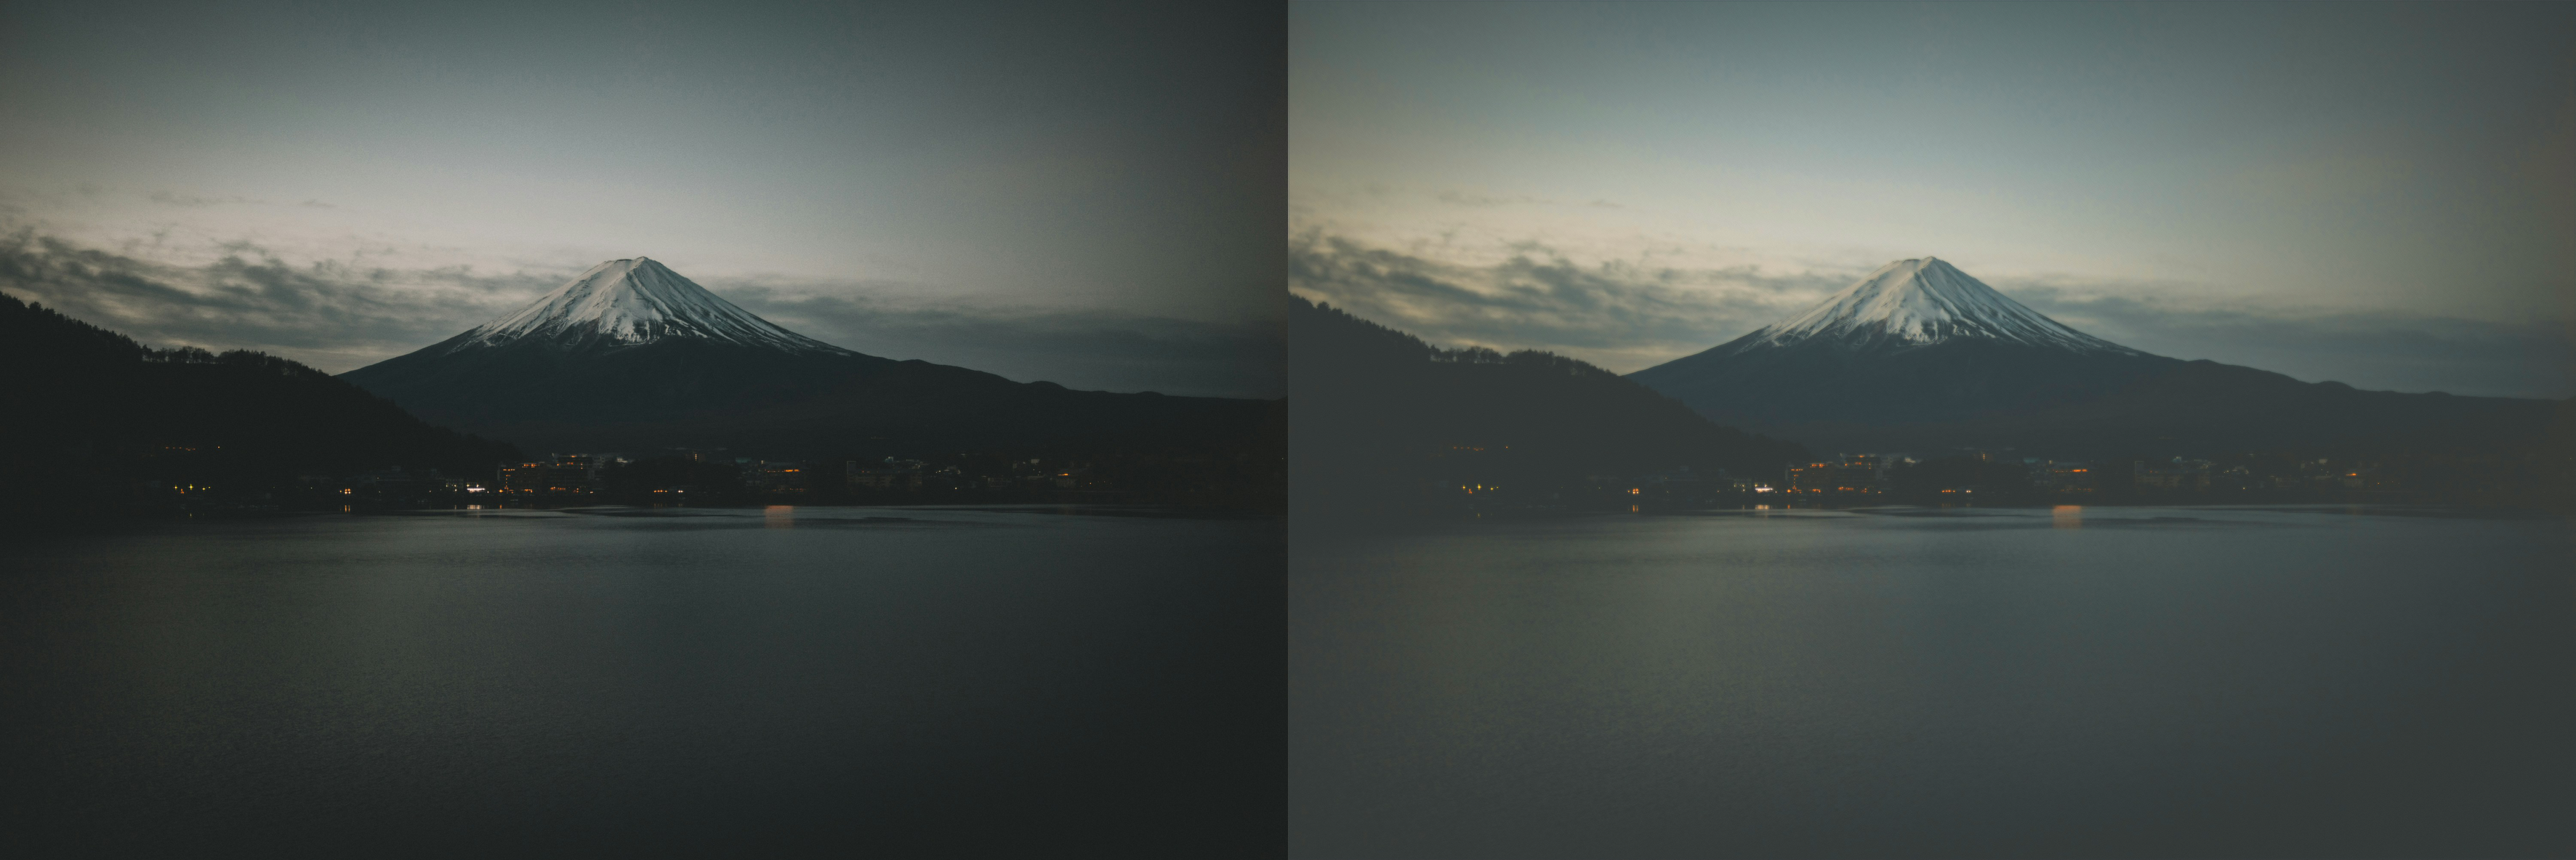
\includegraphics[width=\linewidth]{demo_before_after.png}
\caption{Example output of the web app on a dusk landscape photograph: original (left) and enhanced (right).}
\end{figure}

\begin{figure}[H]
\centering
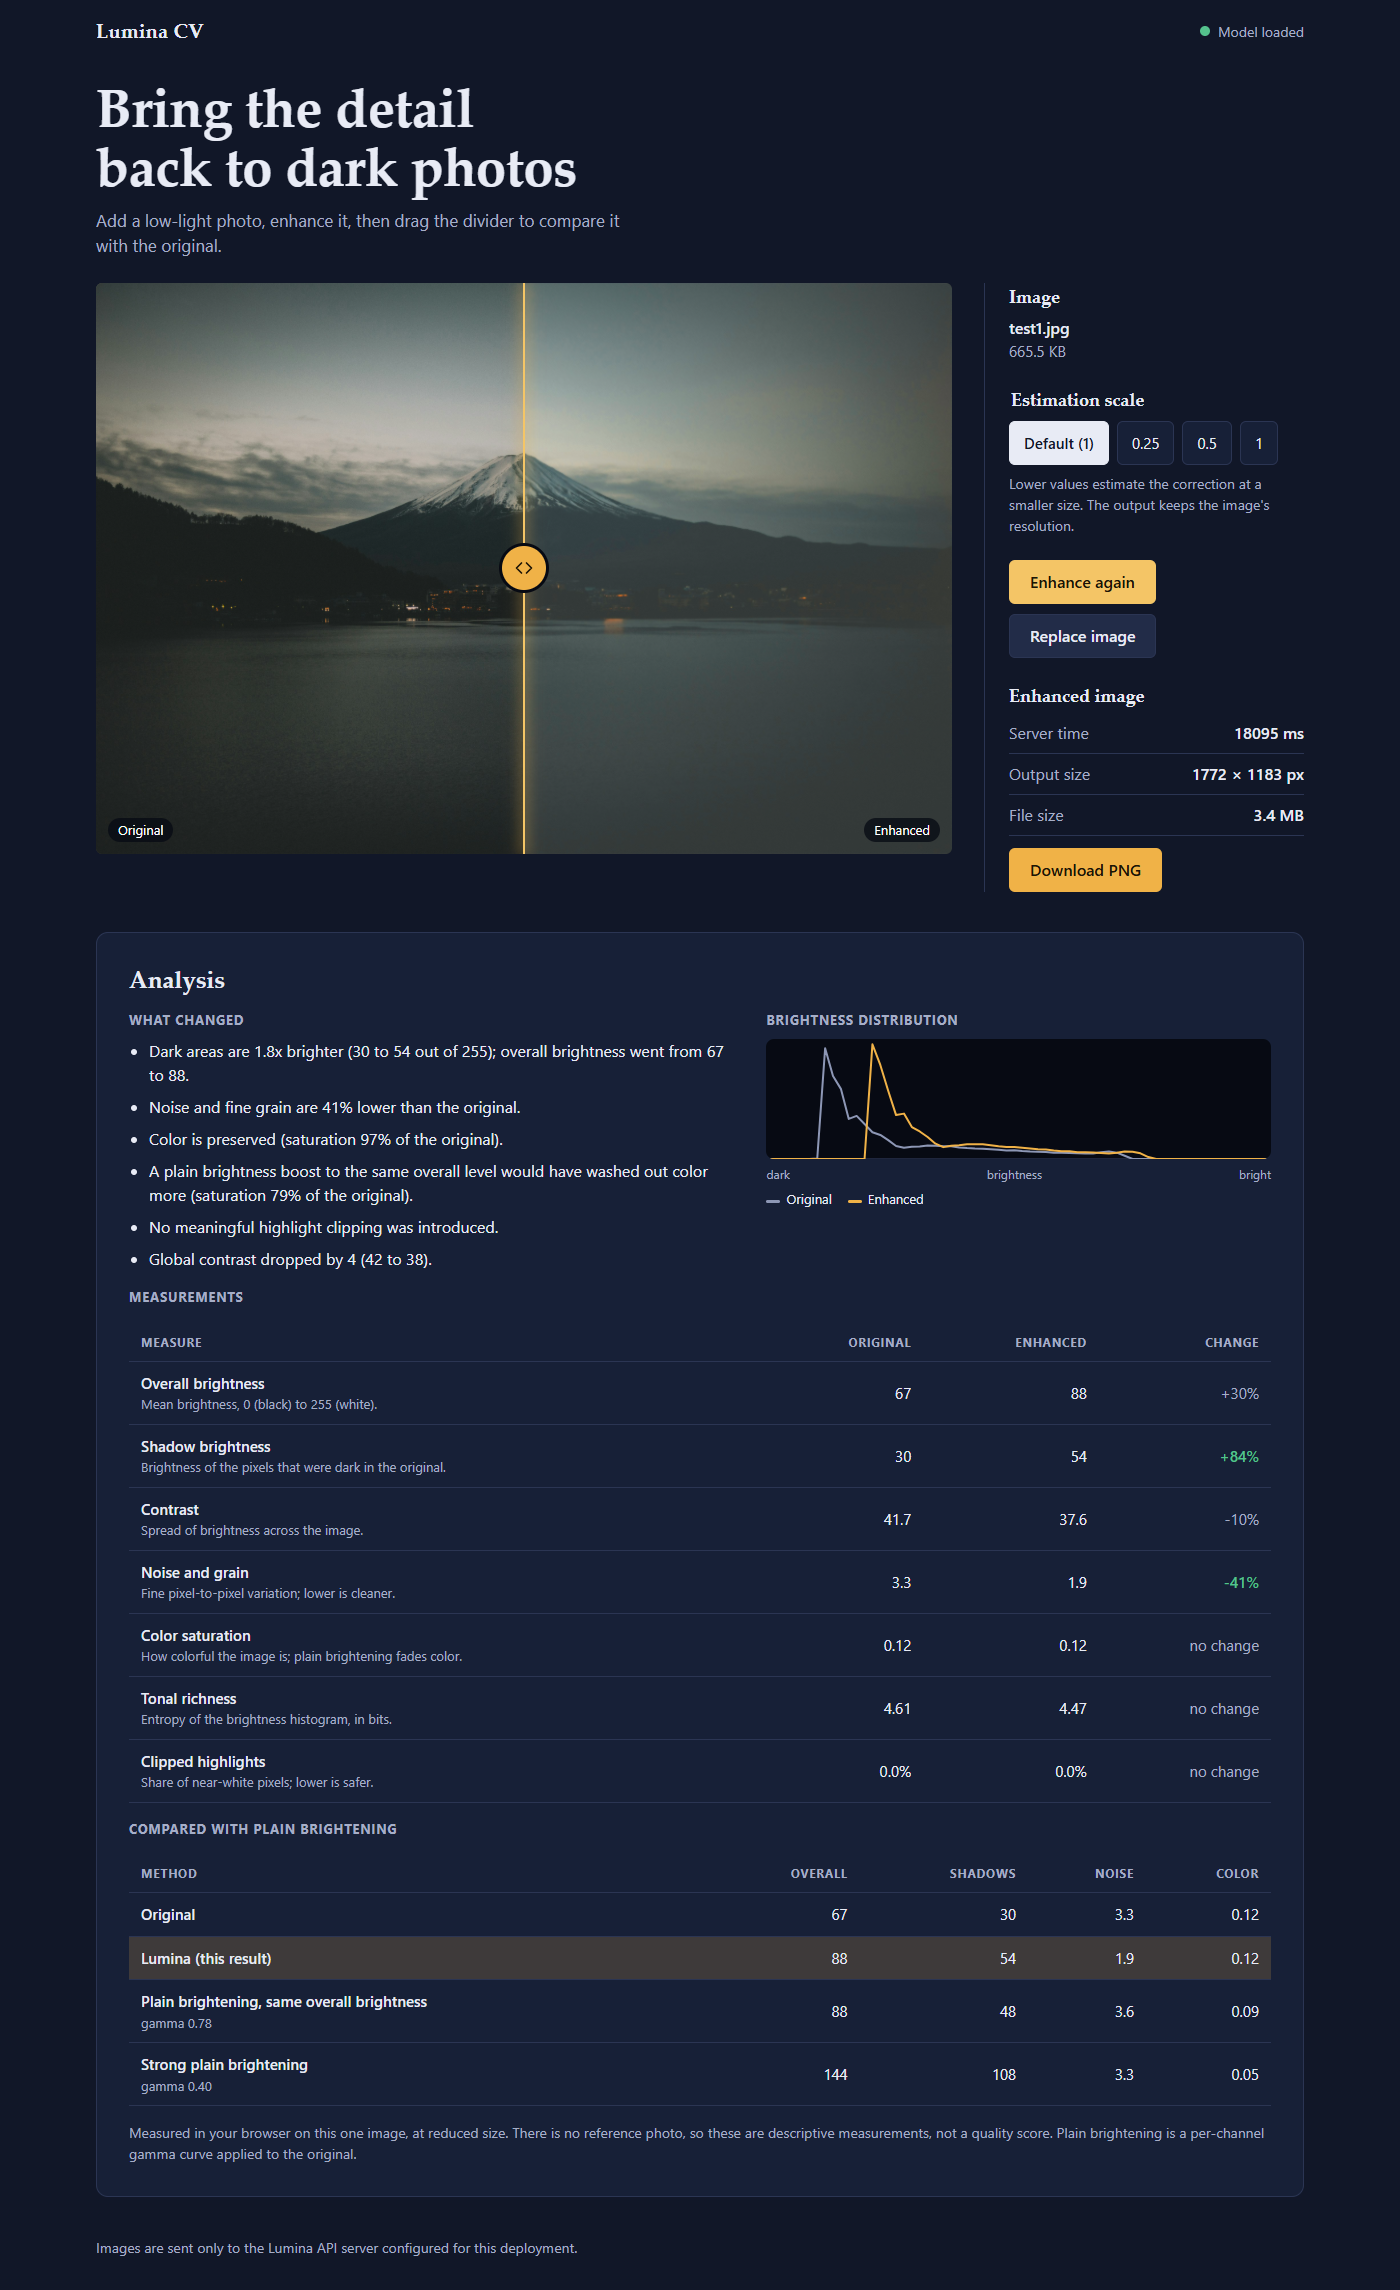
\includegraphics[height=.62\textheight]{ui_analysis_page.png}
\caption{The in-browser Analysis section: brightness, shadows, contrast, noise, saturation, tonal richness, clipping, a histogram and a comparison against plain gamma brightening of matched brightness.}
\label{fig:ui}
\end{figure}

%--------------------------------------------------------------------
\section{Experimental setup}\label{sec:setup}
\textbf{Data.} We use the public LOL dataset~\cite{lol}. The 485 low-light training images are used \emph{without} their references (the objective is zero-reference). The 15 held-out low/normal pairs (\code{eval15}) are used only for evaluation. A procedural synthetic dataset (analytic affine motion with known flow and exposure flicker) was used to train the temporal variant.

\textbf{Metrics.} PSNR and SSIM (11$\times$11 Gaussian window, $\sigma=1.5$) against the normal-light reference; angular error (degrees between RGB vectors, a colour-accuracy measure, lower is better); mean output brightness; fraction of clipped pixels ($Y\ge0.99$); and a flat-region noise estimate (Immerk{\ae}r's method~\cite{immerkaer}), lower is better but biased by texture. All numbers are mean $\pm$ standard deviation over the 15 images. Because the model is deterministic at inference and each setting was trained once (seed 17), the standard deviation reflects variation \emph{between images}, not between training runs.

\textbf{Settings common to all runs.} Adam, learning rate $10^{-4}$, batch size 8, $128\times128$ random crops, 32 channels, 8 curve iterations, loss weights as in Sec.~2.3, CPU training. All trained checkpoints use \code{loss.exposure\_target}\,=\,0.6. Evaluation ran on CPU at full resolution ($400\times600$).

\textbf{Baselines.} Input (no processing); histogram equalisation of the luma channel; and gamma correction $x^{\gamma}$ with $\gamma\in\{0.5,0.4,0.3\}$.

\begin{table}[H]
\centering\small
\begin{tabular}{p{3.3cm}p{3.2cm}p{3.0cm}p{4.2cm}}
\toprule
Run & Training data & Extensions on & Epochs\\
\midrule
\code{lol\_dark\_only} & 485 LOL low-light photos & noise, denoise, edge, chroma, adaptive exp.; \emph{no} temporal & Config said 60; we stopped at 40 and kept a checkpoint every 5 epochs\\
\code{lol/final.pt} (shipped) & same & same & 10 (identical weights to epoch 10 of the above)\\
\code{full} & 96 synthetic procedural pairs & all, including temporal & 40\\
\bottomrule
\end{tabular}
\caption{The training runs for which logs and checkpoints exist.}
\label{tab:runs}
\end{table}

%--------------------------------------------------------------------
\section{Results}
\subsection{Training dynamics}\label{sec:training}
Fig.~\ref{fig:train} shows the loss logs of the two runs for which we have complete logs. The total loss on LOL falls quickly during the first 10 epochs, then slowly (validation total 4.30 $\to$ 2.30 after 40 epochs). The synthetic/temporal run reaches a lower value (1.97), but the two are \emph{not directly comparable}: the data differ and the second run also optimises the temporal term. The decomposition of the validation loss (Fig.~\ref{fig:comp}) shows that the noise, chroma, edge and adaptive-exposure terms dominate the weighted loss, while the baseline spa and colour terms contribute almost nothing. This is a sign that the weights are unbalanced (they were set by hand and never tuned).

\begin{figure}[H]
\centering
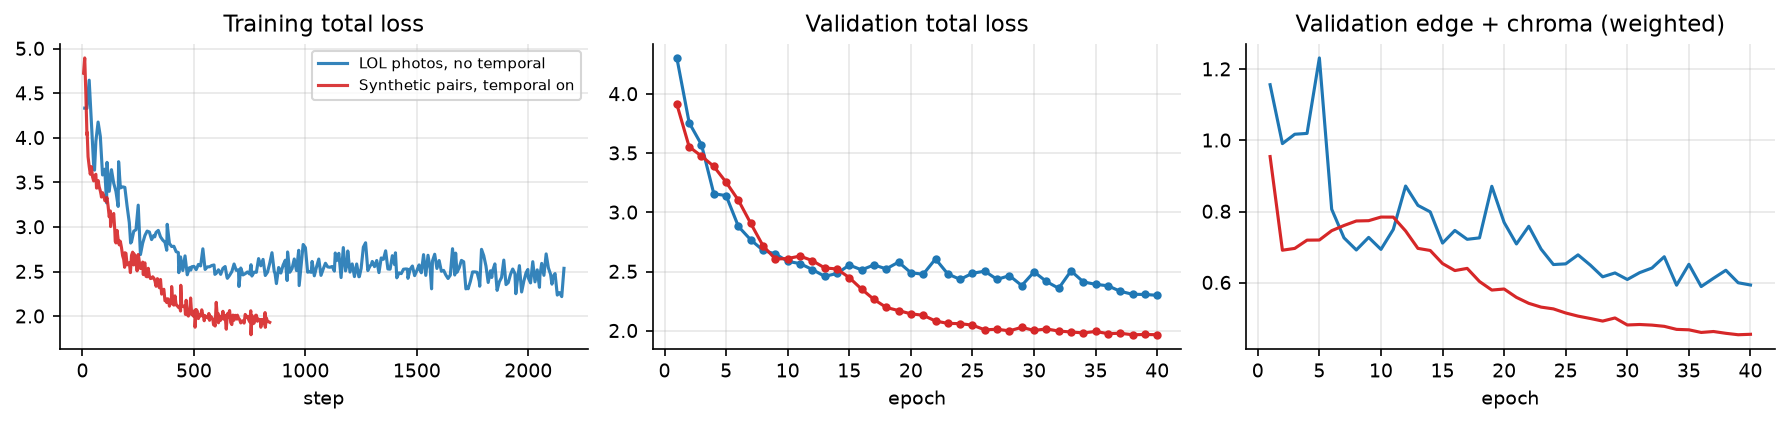
\includegraphics[width=\linewidth]{training_curves.png}
\caption{Left: training loss per logged step. Middle: validation loss per epoch. Right: the weighted edge and chroma terms of the validation loss.}
\label{fig:train}
\end{figure}

\begin{figure}[H]
\centering
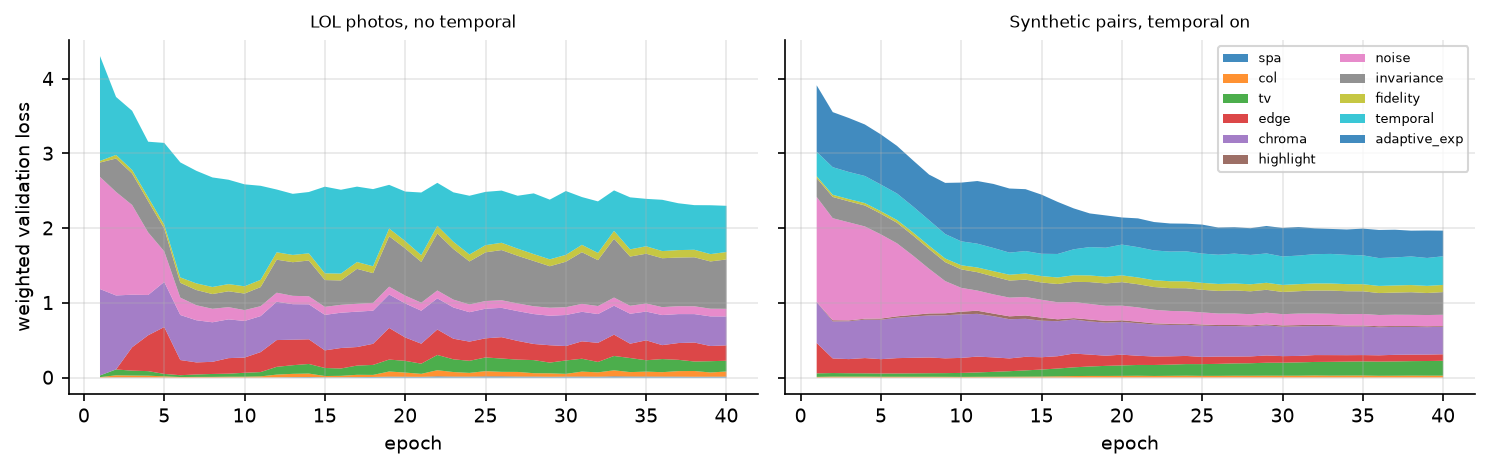
\includegraphics[width=.9\linewidth]{loss_components.png}
\caption{Stacked weighted validation-loss components for both runs.}
\label{fig:comp}
\end{figure}

\subsection{Tuning the training length (checkpoint sweep)}\label{sec:sweep}
The most important ``setting'' we tuned was how long to train. We evaluated each of the eight saved checkpoints of the \code{lol\_dark\_only} run on the 15 held-out pairs (Table~\ref{tab:sweep}, Fig.~\ref{fig:sweep}).

\begin{table}[H]
\centering\small
\begin{tabular}{lcccccc}
\toprule
Setting & PSNR (dB) $\uparrow$ & SSIM $\uparrow$ & Ang.\ err.\ $\downarrow$ & Brightness & Clipped & Noise est.\\
\midrule
Input (no processing) & 7.77 & 0.195 & 10.36 & 0.059 & 0.000 & 0.005\\
Histogram equalisation & 14.24 & 0.419 & 9.98 & 0.512 & 0.008 & 0.053\\
Gamma $\gamma=0.5$ & 12.33 & 0.563 & 9.17 & 0.216 & 0.000 & 0.014\\
Gamma $\gamma=0.4$ & 14.59 & 0.622 & 9.28 & 0.285 & 0.000 & 0.017\\
Gamma $\gamma=0.3$ & \textbf{16.70} & \textbf{0.643} & 9.45 & 0.379 & 0.000 & 0.021\\
\midrule
Ours, epoch 5 & 10.93 & 0.504 & \textbf{7.17} & 0.175 & 0.000 & 0.010\\
Ours, epoch 10 (shipped) & 10.68 & 0.506 & 7.77 & 0.183 & 0.000 & 0.008\\
Ours, epoch 15 & 13.54 & 0.561 & 7.76 & 0.280 & 0.000 & 0.010\\
Ours, epoch 20 & 15.86 & 0.593 & 7.49 & 0.444 & 0.000 & 0.020\\
Ours, epoch 25 & 14.90 & 0.588 & 7.45 & 0.491 & 0.000 & 0.020\\
Ours, epoch 30 & 15.68 & 0.581 & 7.75 & 0.425 & 0.000 & 0.016\\
Ours, epoch 35 & 16.19 & 0.593 & 7.42 & 0.481 & 0.000 & 0.021\\
Ours, epoch 40 & 16.58 & 0.591 & 7.29 & 0.469 & 0.000 & 0.021\\
\bottomrule
\end{tabular}
\caption{Held-out LOL results (mean over 15 image pairs; per-image standard deviations are in Fig.~\ref{fig:sweep}). The mean brightness of the ground-truth references is 0.451. Best value per column among all rows in bold except the angular error, where bold marks the best of our models.}
\label{tab:sweep}
\end{table}

\begin{figure}[H]
\centering
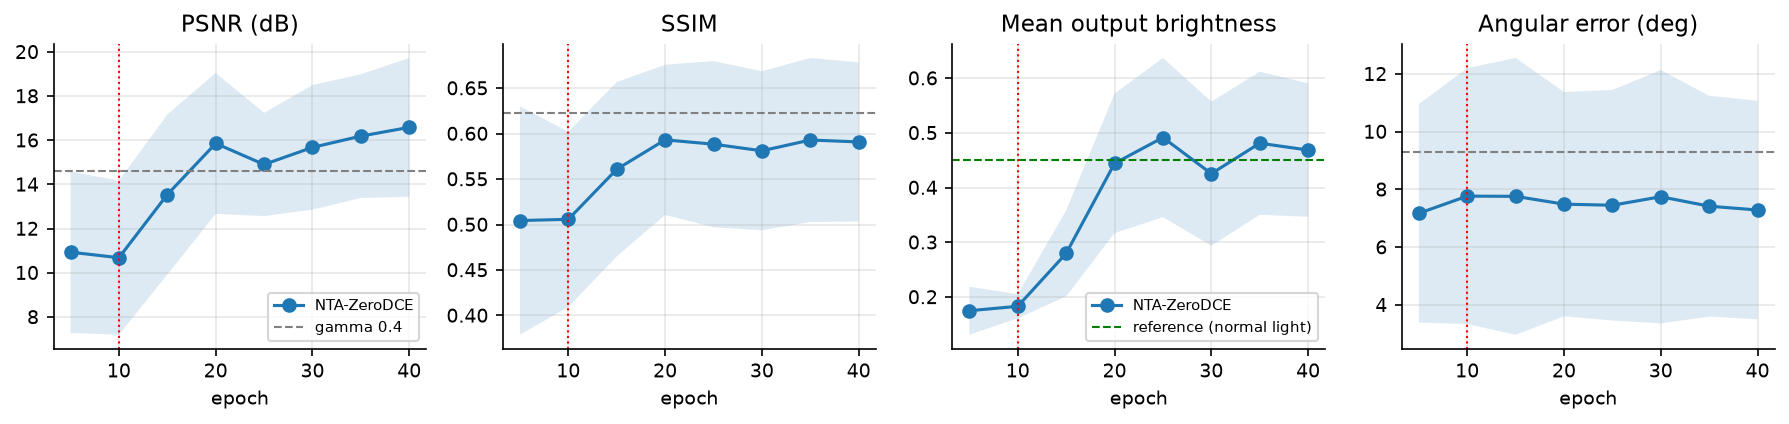
\includegraphics[width=\linewidth]{epoch_sweep.png}
\caption{Metrics versus training epoch. Shaded band: $\pm1$ standard deviation across the 15 images. The dashed grey line is gamma 0.4; in the brightness panel the green dashed line is the average brightness of the ground-truth references. The red dotted line marks the shipped epoch-10 model.}
\label{fig:sweep}
\end{figure}

\textbf{Observations.}
\begin{itemize}[nosep]
  \item PSNR rises from 10.7~dB at epoch 10 to 16.6~dB at epoch 40, with a visible jump between epochs 10 and 20; SSIM plateaus around 0.59 from epoch 20.
  \item Mean brightness climbs from 0.18 to $\approx0.47$ (the reference average is 0.45). The long-trained model therefore does what the benchmark wants on these \emph{very dark} images: it brightens a lot.
  \item Angular error (colour accuracy) is roughly constant, 7.2 to 7.8 degrees, and about 1.5 to 2 degrees better than gamma or histogram equalisation, whose colours shift with brightness.
  \item The noise estimate doubles as brightness rises, as expected: brightening amplifies noise. Histogram equalisation produces by far the noisiest images (0.053).
  \item Clipping stays at essentially zero on these dark images, so this test set cannot reveal the over-brightening problem discussed next.
\end{itemize}

\begin{figure}[H]
\centering
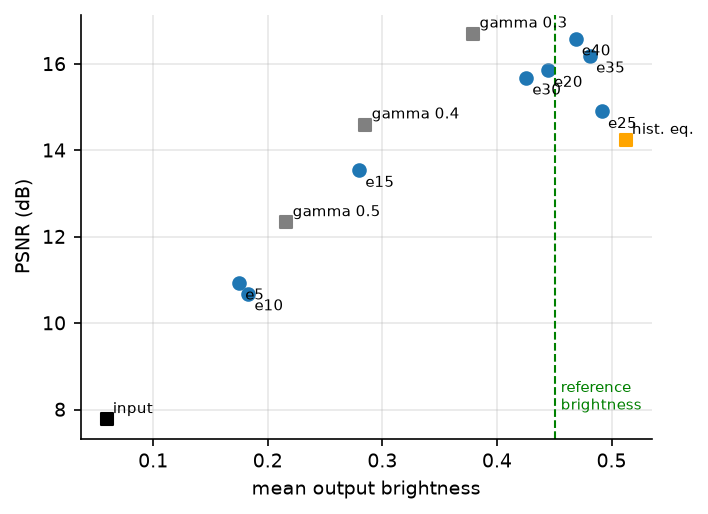
\includegraphics[width=.55\linewidth]{psnr_vs_brightness.png}
\caption{PSNR against mean output brightness. PSNR is largely governed by how close the overall brightness comes to the reference: it increases with brightness for gamma as well as for our checkpoints.}
\end{figure}

\subsection{Why we nevertheless ship the 10-epoch model}
The LOL evaluation images are \emph{extremely dark} (mean 0.06), so a stronger model scores better on them. Ordinary photographs, such as those users upload to the web app, are not that dark. In our manual tests (recorded in the project notes), the checkpoints from epoch 15 onward start to blow out moderately dark photos, and by epoch 25 they wash out almost completely (flat, grey, low-contrast images). Epochs 5 and 10 give natural, moderate enhancement but under-brighten the darkest scenes. This is why the benchmark score and the visual quality move in \emph{opposite} directions, and why \code{lol/final.pt} is the epoch-10 checkpoint. We did not have a held-out set of ordinary photographs, so this finding rests on visual inspection rather than a measured score (see Limitations). Fig.~\ref{fig:qual} shows the progression on LOL images, and the epoch-25 and epoch-40 columns already look bright and low-contrast even though they have the best PSNR.

\begin{figure}[H]
\centering
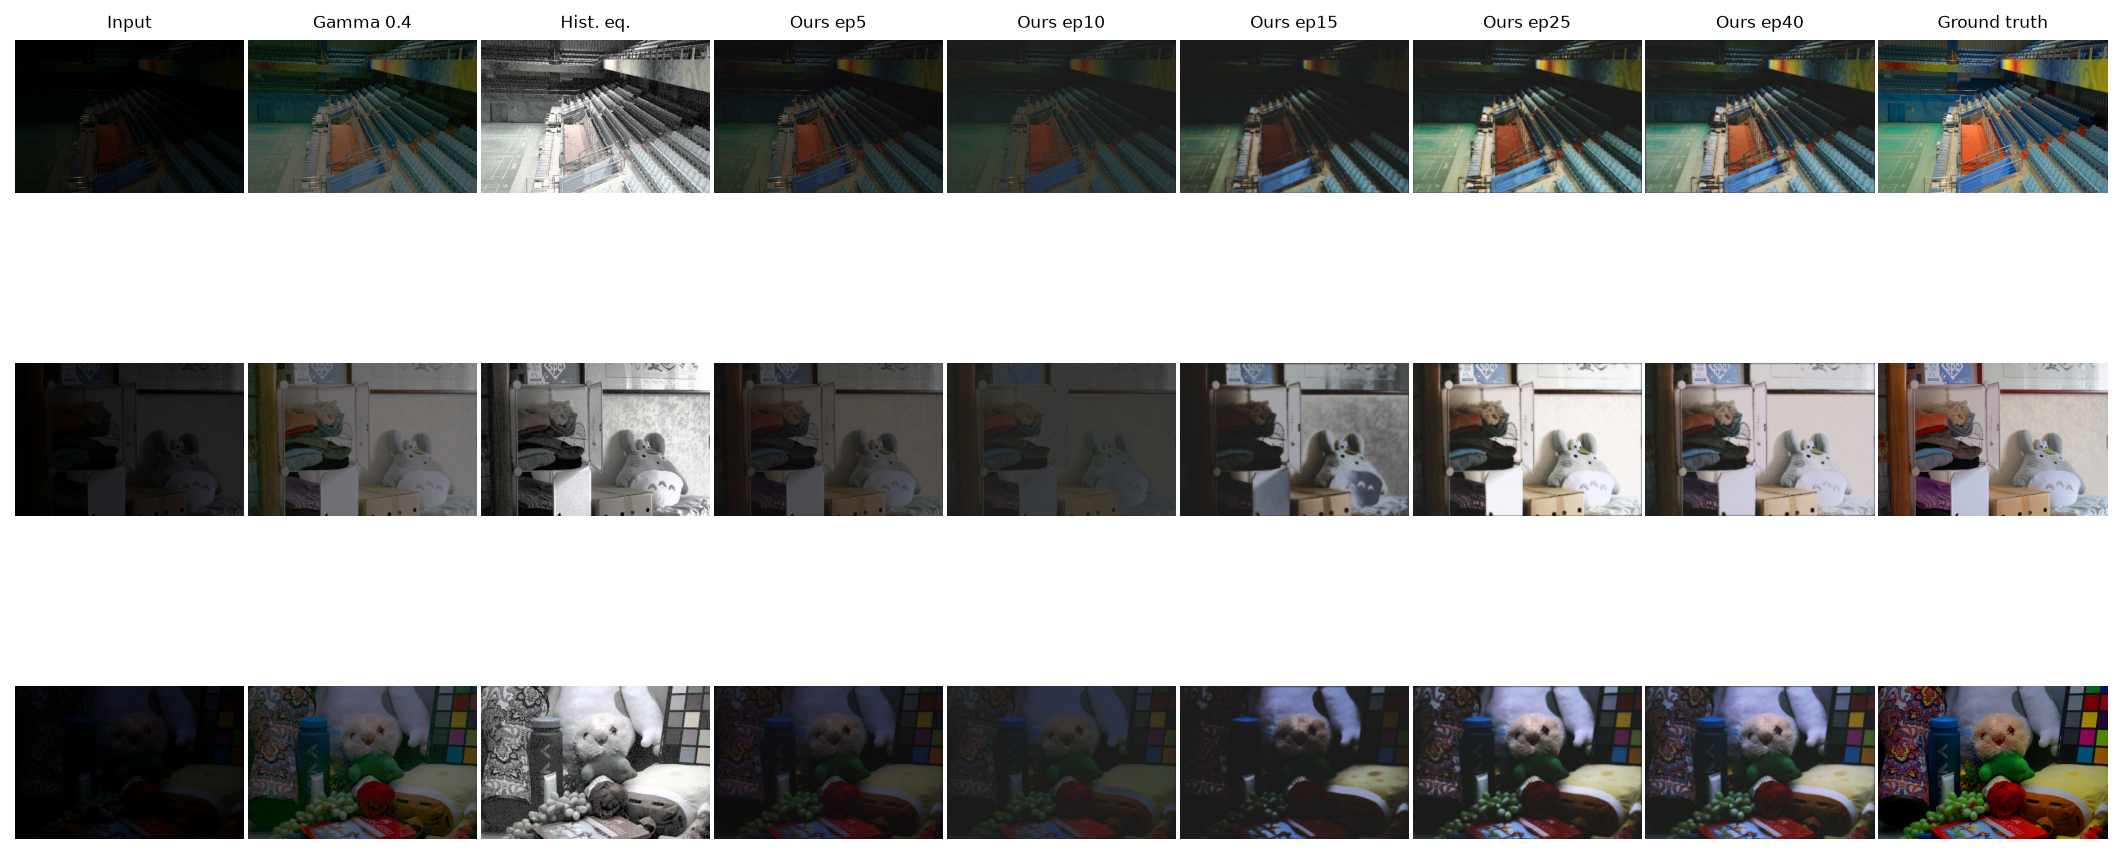
\includegraphics[width=\linewidth]{qualitative_epochs.png}
\caption{Three held-out LOL images processed by the baselines and by different checkpoints. The shipped model (epoch 10) is conservative; later epochs are brighter and score higher on PSNR.}
\label{fig:qual}
\end{figure}

\subsection{Comparison with simple baselines}
\begin{figure}[H]
\centering
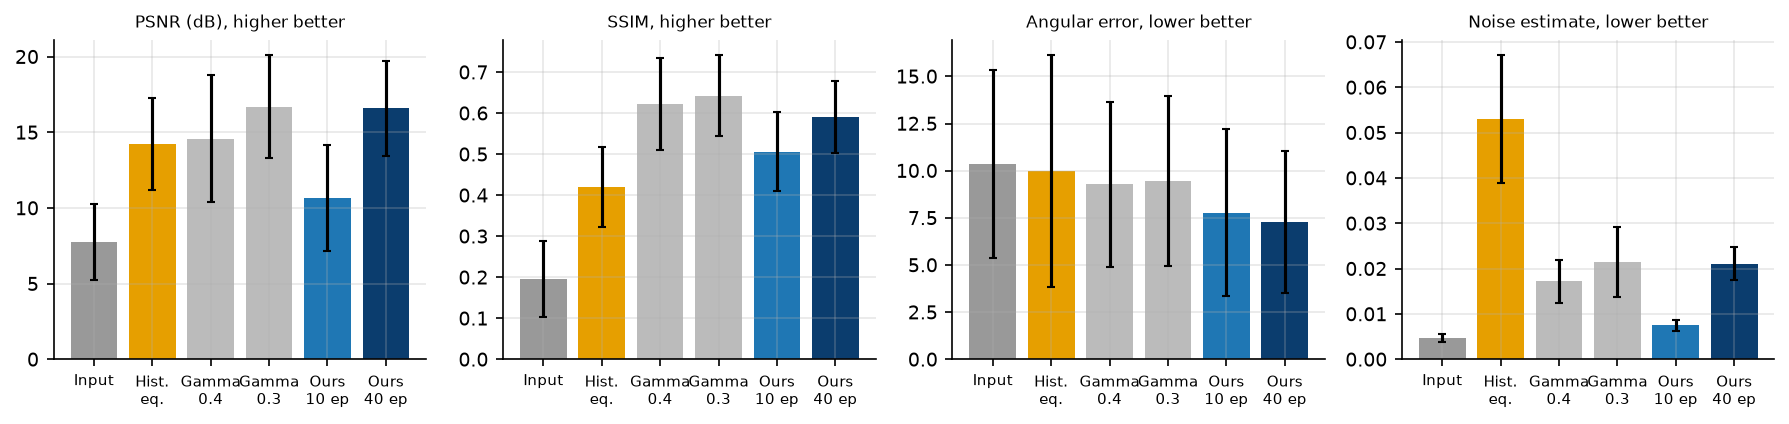
\includegraphics[width=\linewidth]{method_comparison.png}
\caption{Methods compared on the 15 held-out pairs (error bars: standard deviation across images).}
\end{figure}
Honest reading of Table~\ref{tab:sweep}: with respect to PSNR and SSIM, a one-parameter gamma correction ($\gamma=0.3$: 16.7~dB, 0.643) is as good as or better than our best checkpoint (16.6~dB, 0.591). Our model's measurable advantages are (i) a lower angular error (better colour preservation, $7.3$ vs $9.5$ degrees), (ii) no clipping or noise explosion compared with histogram equalisation, and (iii) spatial adaptivity: it does not apply one global curve. Because a zero-reference model is trained without the reference, PSNR is a secondary indicator; but we cannot claim that it beats a tuned global gamma on this benchmark.

\begin{figure}[H]
\centering
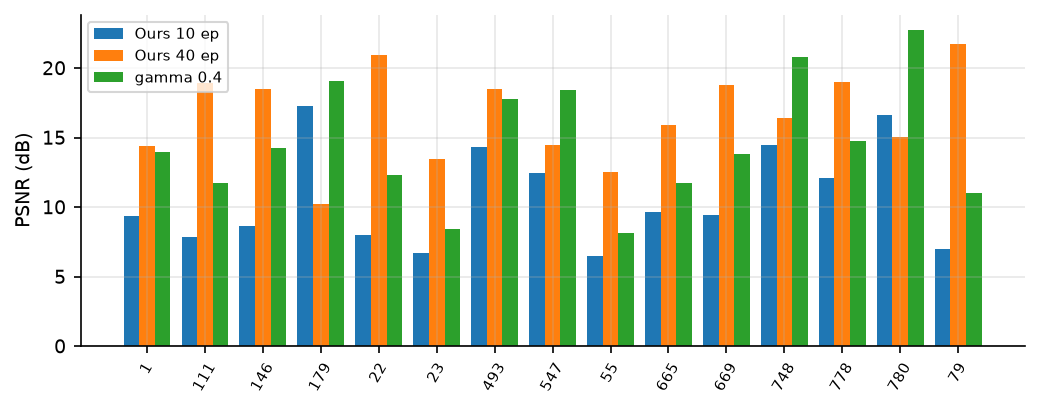
\includegraphics[width=.9\linewidth]{per_image_psnr.png}
\caption{Per-image PSNR for the epoch-10 model, the epoch-40 model and gamma 0.4. The large spread (note the standard deviations of 3 to 4~dB in Table~\ref{tab:sweep}) shows that a 15-image test set is small and results should be read with caution.}
\end{figure}

\begin{figure}[H]
\centering
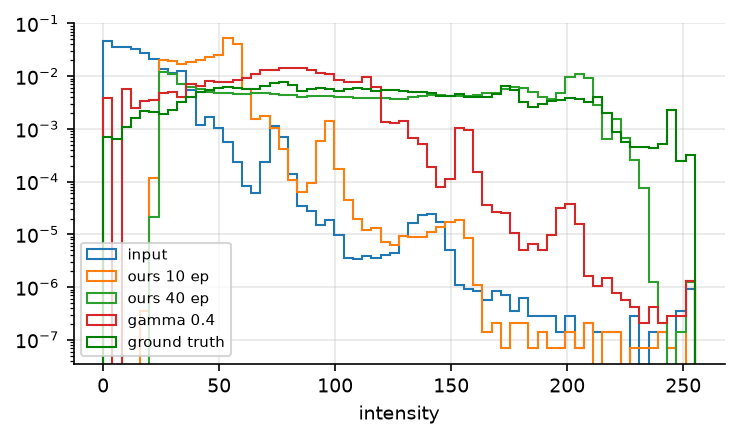
\includegraphics[width=.5\linewidth]{histograms.png}
\caption{Intensity histograms (log scale) over all 15 test images. Inputs concentrate near zero and the shipped model shifts the mass only moderately (mostly below 100). The epoch-40 model's histogram is closer to the ground truth in the mid-tones, but it has no pixels below about 20 and almost none above about 215, i.e.\ reduced contrast with no deep blacks, which is consistent with the washed-out look.}
\end{figure}

\subsection{What the model learns: curves, noise map and denoiser}
Fig.~\ref{fig:internals} visualises the internals for one test image (LOL \code{778}) for the epoch-10 and epoch-40 checkpoints. The mean curve magnitude $|A|$ grows from 0.10 to 0.27 between epoch 10 and 40, which is the mechanism behind the brightening drift: the network simply learns stronger curves. The noise branch predicts a mean $\sigma$ of about 0.019 (10~ep) and 0.016 (40~ep); its map is lowest in the darkest, smooth regions and higher in brighter, textured regions, so it partly reacts to image structure and not only to noise. On this image the residual denoiser improves PSNR from 9.7 to 12.1~dB (10 ep) and from 14.9 to 19.0~dB (40 ep), compared with the curve output alone. This is a single-image observation, not a dataset-level ablation.

\begin{figure}[H]
\centering
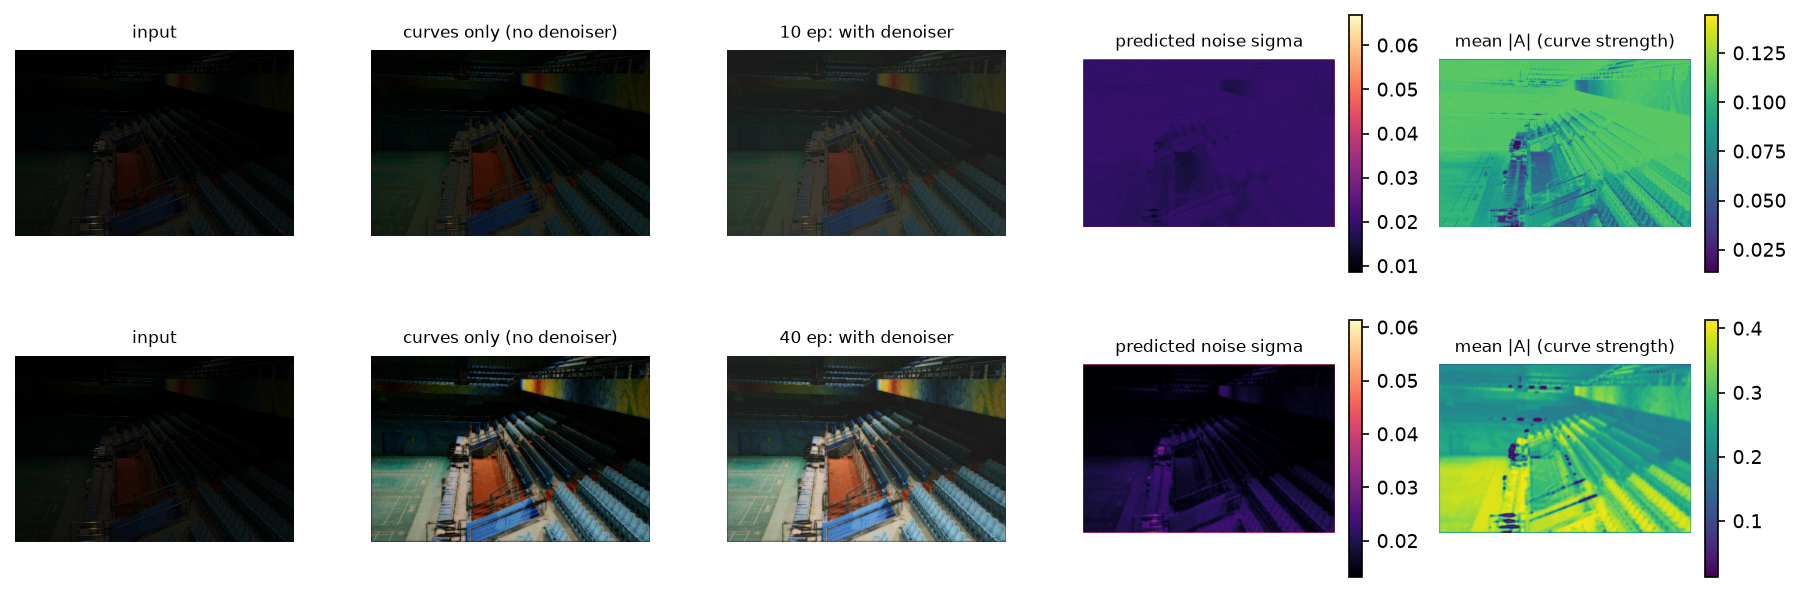
\includegraphics[width=\linewidth]{model_internals.png}
\caption{Inputs, curve-only output, final output, predicted noise map $\sigma$ and mean curve strength for epoch 10 (top) and epoch 40 (bottom).}
\label{fig:internals}
\end{figure}

\subsection{Inference-time setting: \texttt{curve\_scale}}\label{sec:curvescale}
\code{curve\_scale} estimates the curves at a reduced resolution and bilinearly up-samples them, which speeds up inference. We evaluated the shipped model with \code{curve\_scale} $\in\{1,0.5,0.25,0.125\}$ (Table~\ref{tab:cs}, Fig.~\ref{fig:cs}).

\begin{table}[H]
\centering\small
\begin{tabular}{lccccc}
\toprule
\code{curve\_scale} & PSNR & SSIM & Ang.\ err. & CPU s/image\\
\midrule
1.0 & 10.68 & 0.506 & 7.77 & 0.76\\
0.5 & 10.71 & 0.513 & 7.81 & 0.39\\
0.25 & 10.72 & 0.517 & 7.85 & 0.29\\
0.125 & 10.74 & 0.520 & 7.90 & 0.34\\
\bottomrule
\end{tabular}
\caption{Effect of \code{curve\_scale} (shipped model, $400\times600$ images, CPU).}
\label{tab:cs}
\end{table}
Quality is practically unchanged: PSNR and SSIM slightly \emph{increase} (smoother curves), and the colour error increases by 0.1 degrees. Speed roughly doubles at 0.5 and nearly triples at 0.25; below that no further gain appeared. Timings were taken on a shared, unloaded-but-uncontrolled desktop CPU and fluctuate (the 0.125 point is slower than 0.25), so they show the trend rather than precise values.

\begin{figure}[H]
\centering
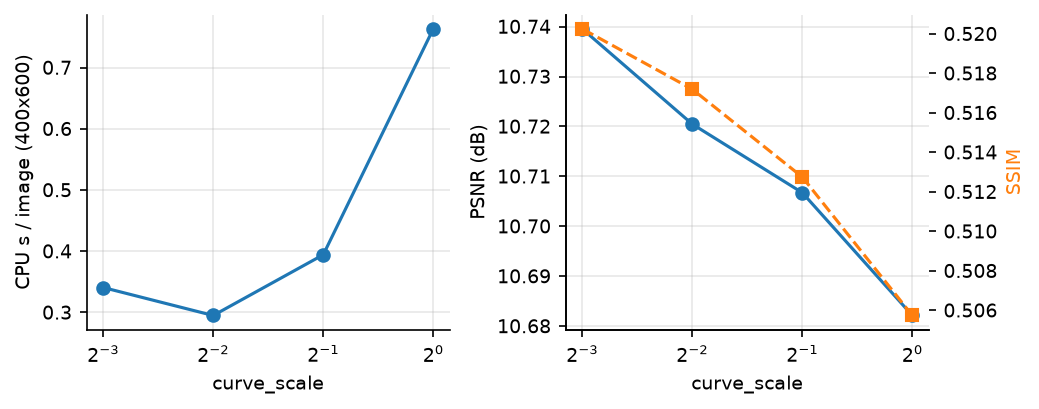
\includegraphics[width=.75\linewidth]{curve_scale.png}
\caption{Speed and quality against \code{curve\_scale}.}
\label{fig:cs}
\end{figure}

\subsection{Other settings we tried}
Table~\ref{tab:tried} lists the remaining decisions, including those taken from the project history and notes rather than from experiments re-run for this report. The right-hand column says what evidence exists.

\begin{table}[H]
\centering\small
\begin{tabular}{p{3.4cm}p{6.0cm}p{5.2cm}}
\toprule
Setting & Outcome & Evidence\\
\midrule
Training data: 96 synthetic procedural images, 40 epochs & Model flattened real photographs to grey; the checkpoint was removed & Project notes (\code{checkpoints/README.md})\\
Training data: LOL low-light photos & Works; basis of all shipped weights & Sec.~\ref{sec:sweep}\\
Adding normal-light and darkened copies to the training set & Did not fix the over-brightening & Project notes (\code{docs/IMPLEMENTATION.md}); not re-run\\
Training length 5 / 10 / 15 / \dots\ / 40 epochs & 10 chosen for visual quality; 40 for benchmark score & Table~\ref{tab:sweep}\\
\code{exposure\_target} 0.6 & Used for \emph{all} shipped checkpoints & Run configs\\
\code{exposure\_target} 0.5 & Now the config default to reduce over-brightening; \textbf{not yet retrained or evaluated} & Commit history; configs\\
Per-step brightness/clipping diagnostics in training logs & Added so drift is visible during training; monitoring only, not a fix & Commit history\\
Temporal term on synthetic pairs & Run trained; lower validation loss, not comparable (different data) & Fig.~\ref{fig:train}\\
\code{curve\_scale} 1 to 0.125 & No quality loss, 2--3$\times$ faster & Table~\ref{tab:cs}\\
13-row ablation matrix (3 seeds) & Defined in \code{configs/ablation\_matrix.py}; \textbf{not run} & No results exist\\
\bottomrule
\end{tabular}
\caption{Settings tried, outcomes and evidence.}
\label{tab:tried}
\end{table}

%--------------------------------------------------------------------
\section{Discussion}
\textbf{Benchmark score versus perceived quality.} The central lesson is that optimising or selecting by held-out PSNR on very dark images would have chosen a 40-epoch model that visually over-brightens. Because the training losses contain an exposure term with a fixed target (0.6), the longer the network trains, the more it pushes every image toward that mean. Stronger curves (Fig.~\ref{fig:internals}) are the mechanism. Early stopping at epoch 10 is a workaround, not a fix.

\textbf{Possible fixes (not yet done).} (i) Retrain with \code{exposure\_target}\,=\,0.5 (already the config default) and compare brightness and clipping; (ii) use the adaptive-exposure target more aggressively so already well-lit images stay unchanged; (iii) build a validation set of ordinary photos and stop on brightness/clipping instead of LOL PSNR; (iv) include a small fraction of well-exposed images with an identity loss.

\textbf{The baselines are strong.} A tuned gamma beats our model on PSNR and SSIM on LOL. The model's value lies in colour fidelity, spatially varying enhancement, a noise-aware path and the fact that it needs no tuning per image, but a fair claim requires a no-reference perceptual metric and a user study, which we did not do.

\textbf{Limitations.}
\begin{itemize}[nosep]
  \item Each setting was trained once with one seed; no confidence intervals over training runs.
  \item The 15-image test set is small; one set (LOL) with very dark images only.
  \item The ablation matrix (value of each extension) was not run, so the individual contribution of noise branch, denoiser, edge, chroma and adaptive-exposure losses is \emph{not} established. The single-image denoiser result is anecdotal.
  \item Loss weights and thresholds are untuned starting values; synthetic noise is a Gaussian approximation.
  \item The ``ordinary-photo over-brightening'' finding rests on visual inspection of a few images.
  \item Video/temporal consistency was implemented and unit-tested, but no video benchmark was run.
  \item Checkpoints use PyTorch pickle serialisation: load only trusted files. The API has no authentication.
\end{itemize}

%--------------------------------------------------------------------
\section{Conclusion}
We delivered a complete low-light enhancement system: a small, noise-aware zero-reference model, a robust API, and a web app with built-in analysis. Our experiments on checkpoint selection show a clear tension between a benchmark metric and natural-looking results, and we chose the conservative 10-epoch model for deployment. Honest next steps are to run the ablation matrix, test the lower exposure target, evaluate on ordinary photographs and on video, and compare against other zero-reference methods.

\section*{Team}
\begin{center}
\begin{tabular}{ll}
\toprule
Name & Roll number\\
\midrule
Jatin Purbia & B23CH11022\\
Sharana Gouda Lakshetty & B23CH1042\\
Rahul Ahuja & B23CH1037\\
\bottomrule
\end{tabular}
\end{center}

\section*{Reproducing the numbers}
All figures and tables in Sec.~4 were produced by running the committed checkpoints in \code{core/checkpoints/} on the 15 LOL evaluation pairs in \code{core/data/LOL/eval15/} (CPU, full resolution). The training-curve figures read \code{core/runs/*/metrics.csv} and \code{val\_metrics.csv}.

\begin{thebibliography}{9}
\bibitem{zerodce} C.~Guo, C.~Li, J.~Guo, C.~C.~Loy, J.~Hou, S.~Kwong, R.~Cong. Zero-Reference Deep Curve Estimation for Low-Light Image Enhancement. \emph{CVPR}, 2020.
\bibitem{zerodcepp} C.~Li, C.~Guo, C.~C.~Loy. Learning to Enhance Low-Light Image via Zero-Reference Deep Curve Estimation. \emph{IEEE TPAMI}, 2021.
\bibitem{lol} C.~Wei, W.~Wang, W.~Yang, J.~Liu. Deep Retinex Decomposition for Low-Light Enhancement. \emph{BMVC}, 2018.
\bibitem{dis} T.~Kroeger, R.~Timofte, D.~Dai, L.~Van Gool. Fast Optical Flow using Dense Inverse Search. \emph{ECCV}, 2016.
\bibitem{immerkaer} J.~Immerk{\ae}r. Fast Noise Variance Estimation. \emph{Computer Vision and Image Understanding}, 1996.
\bibitem{ssim} Z.~Wang, A.~C.~Bovik, H.~R.~Sheikh, E.~P.~Simoncelli. Image Quality Assessment: From Error Visibility to Structural Similarity. \emph{IEEE TIP}, 2004.
\bibitem{lai} W.-S.~Lai et al. Learning Blind Video Temporal Consistency. \emph{ECCV}, 2018.
\end{thebibliography}

\appendix
\section{Hyperparameters of the shipped configuration}
\begin{table}[H]
\centering\small
\begin{tabular}{ll}
\toprule
Parameter & Value\\
\midrule
Channels / curve iterations & 32 / 8\\
Noise / denoiser channels & 16 / 16\\
$\sigma_{\max}$, residual scale & 0.2, 0.1\\
Gain window, gain range & 5, [1, 8]\\
Loss weights (spa, exp, col, tv) & 1, 10, 5, 200\\
Loss weights (edge, chroma, highlight, noise, invariance, fidelity, temporal) & 20, 20, 20, 20, 10, 1, 10\\
Noise synthesis & $a\in[0,0.01]$, $b\in[0,0.02]$\\
Optimiser & Adam, $\beta=(0.9,0.999)$, weight decay $10^{-4}$\\
Learning rate, batch, crop & $10^{-4}$, 8, 128\\
Gradient clipping & 0.1\\
Seed & 17\\
Exposure target (shipped weights) & 0.6\\
Exposure target (current config default) & 0.5 (not retrained)\\
\bottomrule
\end{tabular}
\end{table}

\end{document}
